\chapter{A cosmological mechanism for depopulating dark matter}
\label{chap:wimpdecay}

\chapterquote{In order to make an apple pie from scratch, you must first create the universe.}%
{Carl Sagan, 1934--1996}

One of the notable concerns with neutralino dark matter in the MSSM is the familiar bino-like overabundance at early times, due to feeble annihilation rates. In this chapter, we describe a cosmological mechanism for reducing the abundance substantially through temporary decays. These early decays can arise from a spontaneously broken symmetry, which is then appropriately restored as the universe cools to stabilize the dark matter\footnote{An approach has been considered in \cite{RN739}, using additional auxiliary dark sector fields that require a specific mass arrangement.}.

In reference \cite{RN802} we discuss how this can be applied to a model of fermionic dark matter based on the inert \acrshort{2hdm} model \cite{RN602}, in which DM particles are odd under an imposed $Z_2$ symmetry and SM particles are even. In this case, at high temperatures the $Z_2$ symmetry is broken temporarily and then restored at lower temperatures, accounting for a phase in which the dark matter abundance is reduced through decays. Here instead we introduce a generic discussion of how we can exploit this mechanism in a model-independent fashion before exploring how this could be applied to the MSSM. In particular, dark matter in the MSSM can be destabilized in an analogous way through temporary $R$-Parity violation, a discrete $Z_2$ symmetry that prevents decay of the lightest neutralino to SM particles.

\section{A closer look at the WIMP relic density: The Boltzmann Equation}
\label{sec:boltzmann}

In the generic WIMP paradigm, dark matter particles were in thermal equilibrium with the constituents of the Universe in its early history. The departure from thermal equilibrium, where the dark matter decouples from the plasma occurs when the expansion rate of the Universe, $H$, overtakes the interaction rate of the heavy particles, $\Gamma$. We refer to this time in cosmological history as the WIMP \textit{freeze-out}, since the (co-moving) density of particles remains constant after decoupling - assuming it is kept stable (or is very long-lived compared to the age of the Universe) until the present day. If these particles were kept in equilibrium, they would have indeed been thermally suppressed by the factor $e^{-m/T}$. The Boltzmann equation for WIMP particles $\chi$ describing this process can be written as \footnote{Derivations of this equation in the form of Eq. \ref{eqn:boltzmann} can be readily found in \cite{RN785, RN682, RN681}.}:
\begin{equation}
a^{-3} \frac{d \left( n_{\chi} a^3\right)}{dt} = \left \langle \sigma v \right \rangle \left[ (n^{\text{EQ}}_{\chi})^2-n_{\chi}^2 \right].
\label{eqn:boltzmann}
\end{equation}
In the above, $a$ is the scale factor as usually defined through the Hubble expansion constant as $H \equiv \dot{a}/a$ and $n_{\chi}$ and $n^{\text{EQ}}_{\chi}$ are the dark matter number density and equilibrium number density, respectively. $\left \langle \sigma v \right \rangle$ is the thermally-averaged cross section, summed over all annihilation channels. It typically becomes convenient to factor out the effects of the universal expansion by using the number density of particles per co-moving volume. For this sake, let us then define the quantities
\begin{equation}
Y_{\chi} \equiv \frac{n_{\chi}}{s}, \qquad x \equiv \frac{m_\chi}{T}.
\end{equation}
$s=(2\pi^2/45)g_{*s}T^3$ is the entropy density, dominated by relativistic contributions, where
\begin{equation}
g_{*s}=\sum_{i=\text{bosons}} g_i \left( \frac{T_i}{T}\right)^3 + \frac{7}{8} \sum_{i=\text{fermions}} g_i \left( \frac{T_i}{T}\right)^3.
\end{equation}
In the early universe, at equilibrium, most species had identical temperatures, so $g_{*s}=g_*$. We will ignore dependence of $g_*$ on temperature, to good approximation. In general, the thermally-averaged cross section has dependence on velocity $v$, $\sigma v \propto v^p$ where $p=0$ is $s$-wave annihilation, $p=2$ is $p$-wave annihilation. Since $\left \langle v \right \rangle \sim T^{1/2}$, we parameterize the cross section as
\begin{equation}
\left \langle \sigma v \right \rangle \equiv \sigma_0 (T/m_{\chi})^n = \sigma_0 x^n,
\end{equation}
where $n=0$ corresponds to $s$-wave annihilation, $n=1$ for $p$-wave and so on. Changing from $t$ to the variable $x$, we require the Jacobian $dx/dt=Hx$. Hence, with all this we can write the Boltzmann equation for the abundance $Y_{\chi}$:
\begin{equation}
\frac{dY_{\chi}}{dx} = -\frac{\lambda}{x^{n+2}} \left[ Y_{\chi}^2-(Y^{\text{EQ}}_{\chi})^2 \right],
\label{eqn:YBoltz}
\end{equation}
where
\begin{equation}
\lambda = \left[ \frac{x s_{\chi} \left \langle \sigma v \right \rangle}{H_{\chi}}\right]_{x=1}.
\end{equation}
In the above, we have implied $s_{\chi}=(2\pi^2/45)g_{*}m^3_{\chi}$ and $H_{\chi}=(\pi^2g_{*}/90)^{1/2} (m^2_{\chi}/M_P)$ as the entropy density and Hubble expansion rate, respectively, both evaluated at $T=m_{\chi}$. For an $s$-wave process ($n=0$), $\lambda$ is constant, but in general higher partial waves mean that $\left \langle \sigma v \right \rangle$ may have some temperature dependence. We will ignore any temperature dependence on the thermally averaged cross-section. Similarly, it is safe for our purposes to ignore changes in $g_*$ with respect to temperature.

Initially, at $x \ll 1$, the relic abundance $Y_{\chi}$ approximately tracks the equilibrium abundance $Y^{\text{EQ}}_{\chi}$, which we can write as $Y_{\chi}(x)=Y^{\text{EQ}}_{\chi}(x)+\delta \approx Y^{\text{EQ}}_{\chi}(x)$. These equilibrium abundances have the simple forms:
\begin{eqnarray}
Y_{\chi}^{\text{EQ}}(x)=\left\lbrace
\begin{array}{ll}
\frac{45}{2\pi^4}\left(\frac{\pi}{8}\right)^{1/2}\frac{g_{\chi}}{g_{*}}x^{3/2}{e}^{-x}~, & m_{\chi} \gg T, \\
	\frac{45\zeta(3)}{2\pi^4}\frac{g_{\text{eff}}}{g_{*}} \simeq 0.278\frac{g_{\text{eff}}}{g_{*}}~, & T \gg m_{\chi}, \\ 
\end{array} 
\right.
\label{eqn:equilbabund}
\end{eqnarray}
where $g_{eff}=g_{\chi}$ $(g_{eff}=3g_{\chi}/4)$ measures the degrees of freedom for bosonic (fermionic) dark matter. For relativistic particles, clearly $Y_{\chi}^{\text{EQ}}$ remains constant up until the dark matter becomes relativistic (or $x>1$). For non-relativistic dark matter, $Y_{\chi}^{\text{EQ}}$ becomes exponentially suppressed at later times and the $Y_{\chi}$ will dominate completely. At this point, the dark matter scatterings are so rare that they cannot maintain equilibrium in the thermal bath. At close to freeze-out, the departure from equilibrium is significant and $Y_{\chi} \approx \delta \gg Y_{\chi}^{\text{EQ}}$ ($x \sim x_f$) where
\begin{equation}
\delta(x) \approx \frac{x^{n+2}}{2\lambda}.
\label{eqn:delta}
\end{equation}
For $x \gg x_f$ one can then drop the equilibrium yield from Eq. \ref{eqn:YBoltz} and integrate from the freeze-out to the present day, $x_{\infty}$ to give:
\begin{equation}
Y^{\infty}_{\chi} \approx \frac{(n+1)Y_{\chi}(x_f)x^{n+1}_f}{Y_{\chi}(x_f)\lambda + (n+1)x^{n+1}_f},
\label{eqn:Yxf}
\end{equation}
where $Y_{\chi}(x_f)=\delta(x_f)$ for non-relativistic dark matter. For relativistic dark matter at decoupling, $Y_{\chi}(x_f)=Y_{\chi}^{\text{EQ}}$. Typically, the correct relic abundance when the decoupling is non-relativistic occurs when $x_f \sim \mathcal{O}(10)$, and so in summary, the final yield of dark matter for these situations are:
\begin{eqnarray}
Y^{\infty}_{\chi}=\left\lbrace
\begin{array}{ll}
\frac{(n+1)x^{n+1}_f}{\lambda}~, & \text{non-relativistic} \\
0.278\,(0.208)\frac{g_{\text{eff}}}{g_{*}}~, & \text{relativistic bosons (fermions)} \\ 
\end{array} 
\right.
\label{eqn:Ychiinf}
\end{eqnarray}
Since we typically have $\lambda \gg 1$, the relativistic decoupled dark matter is several orders of magnitude higher than the non-relativistic decoupling. This is finally recast into the form of the fraction of present-day critical density from $\chi$,
\begin{equation}
\Omega_{\chi} = \frac{m_{\chi}Y^{\infty}_{\chi} s_0}{3 H^2_0 M^2_P},
\end{equation}
where $s_0=2891.2\,\text{cm}^{-3}$ and $H_0=100\,h\,\text{km}\, \text{s}^{-1}\,\text{Mpc}^{-1}$ $(h=0.673)$ are the present day entropy density and Hubble expansion rate \cite{RN493}.

\begin{center}
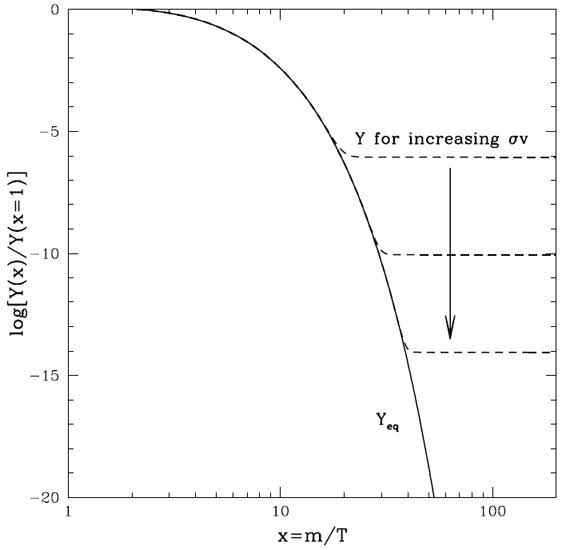
\includegraphics[width=0.6\linewidth]{figures/KolbTurner.jpg}
\captionof{figure}[WIMP freeze-out abundance.]{The typical `freeze-out' description of a non-relativistic DM species from equilibrium with the surrounding plasma at about $x_f \sim \mathcal{O}(10)$. The dashed line shows the abundance of DM per comoving volume element, whilst the solid line is the equilibrium abundance. Adapted from \cite{RN681}.}
\label{fig:KolbTurner}
\end{center}

\section{Decays from a cosmological phase transition}
\label{sec:Decays}

Let us suppose that there is a symmetry stabilizing the DM up to a time $x_a$, in which this symmetry is spontaneously broken. This cosmological phase transition persists until $x_b$, in which the symmetry is then restored. Hence, during the instability phase $x \in [x_a , x_b]$, the DM is permitted to decay. As seen in the previous section, we would require that the dark matter be non-relativistic for some, if not all, of the instability phase in order to suppress inverse decays that would repopulate the dark matter. The Boltzmann equation in Eq. \ref{eqn:YBoltz} then gets modified with a decay term\footnote{In general, we should include the thermally-average decay width $\langle \Gamma_{\chi} \rangle= \Gamma_{\chi}K_1 (x)/K_2 (x)$ where $\Gamma_{\chi}$ is the zero-temperature width and $K_n(x)$ are the modified Bessel functions \cite{RN782,RN784,RN783}. For non-relativistic DM, this has the asymptotic form $K_1(x)/K_2(x)=1-3/(2x)+\mathcal{O}(x^{-2})\, (x \gg 1)$ and so can be approximated by the zero-temperature width, whilst for relativistic dark matter is $K_1(x)/K_2(x)=x/2+\mathcal{O}(x^2)\, (x \ll 1)$ (see Appendix \ref{app:specfunc}). Hence, we neglect DM decay before it becomes non-relativistic since they are highly suppressed.}:
\begin{equation}
	\frac{dY_{\chi}}{dx}=-\frac{2\Gamma_{\chi}x}{g_{\chi}H_{\chi}}\left[Y_{\chi}-Y_{\chi}^{\text{EQ}}\right]-\frac{\lambda}{x^{n+2}}\left[Y_{\chi}^2-\left(Y_{\chi}^{\text{EQ}}\right)^2\right]\;.
    \label{eqn:YBoltzDecay}
\end{equation} 
Here $\Gamma_{\chi}$ is the decay width of the DM particle.

Before we consider the effects of decays on dark matter density, we must first comment on the consequence of entropy production during the phase transition, which can also dilute the dark matter density when it is a first-order transition \cite{RN787,RN786}. Since the phase transition occurs well above $T=1$ GeV, we can neglect entropy production from particle decoupling, or in other words, we can assume $g_*$, the number of relativistic degrees of freedom, is approximately constant. The change in entropy can then be parameterized by a dilution factor (as in \cite{RN787}) where $\gamma \equiv s(x_f)/s(x_i)$ such that the final density changes as
\begin{equation}
	Y^{\infty}_{\chi} \rightarrow \frac{Y^{\infty}_{\chi}}{\gamma}, \quad \Omega_{\chi} \rightarrow \frac{\Omega_{\chi}}{\gamma},
\end{equation}
where $\gamma > 1$. Here, $x_i$ and $x_f$ represent the beginning and after the phase transition, respectively. This is valid for the case where the dark matter density is much larger compared to its equilibrium abundance, $Y_{\chi} \gg Y^{EQ}_{\chi}$, as is the case after freeze-out and annihilations are negligible compared to decays. However this also holds for DM yields that are close to their equilibrium value, $Y_{\chi} \sim Y^{EQ}_{\chi}$. In many general cases, the analytical solutions are not available.

The effect of the DM decays depends on when this instability takes place relative to the time of freeze-out, and the size of the decay rate $\Gamma_{\chi }$. Let us consider (4) separate scenarios:
\begin{enumerate}[label=(\arabic*)]
\item \textit{Freeze-out precedes first phase transition}, $x_f \ll x_a$. Here we expect a significant change in the final density of dark matter. In Eq. \ref{eqn:YBoltzDecay}, the equilibrium yield would be exponentially suppressed, which then resembles the Bernoulli equation and is analytically solvable in terms of the incomplete Gamma function, $\Gamma(\alpha,x)$:
\begin{align}
	Y_\chi(x_b) &= \frac{ Y_{\chi }(x_a)    e^{-\frac{\Gamma _{\chi }}{2 H_{\chi }} x_b^2}}{ e^{-\frac{\Gamma_{\chi}}{2 H_\chi}x_a^2}  + \lambda\, Y_\chi(x_a)\,\frac{1}{2} \left(\frac{\Gamma _{\chi }}{2 H_{\chi }}\right)^{\frac{n+1}{2}}
	\left[
		\Gamma \left(\frac{-1-n}{2},\frac{ \Gamma _{\chi }}{2 H_{\chi }} x_a^2\right)
 - \Gamma \left(\frac{-1-n}{2},\frac{ \Gamma _{\chi }}{2 H_{\chi }} x_b^2\right)
\right]}\\
&\approx
\frac{  Y_{\chi }(x_a)    e^{-\frac{\Gamma _{\chi }}{2 H_{\chi }} (x_b^2-x_a^2)}}{ 1 + \lambda\,Y_\chi(x_a) \,\frac{  H_\chi}{\Gamma_\chi} 
	\left[
		\frac{1}{x_a^{3+n}}
		-\frac{e^{-\frac{\Gamma_\chi}{2 H_\chi} (x_b^2-x_a^2)}}{x_b^{3+n}}
\right]}.
\label{eqn:Yxb1}
   \end{align}
The second line uses a leading-order asymptotic expansion for the incomplete Gamma function, for fixed $\alpha$ and large $x$ (this is detailed in appendix \ref{app:specfunc}). The scattering cross-section is present in Eq. \ref{eqn:Yxb1} through the matching condition, i.e. $\lambda Y_{\chi}(x_a) \approx (n+1)x_f^{n+1}$ for non-relativistic freeze-out at $x_f$. The exponential suppression factor $\Gamma_{\chi}(x^2_b - x^2_a)/H_{\chi}$ in Eq. \ref{eqn:Yxb1} has a simple intuitive explanation. The reduction of dark matter density is defined through the decay rate of dark matter per the universal expansion rate multiplied by the decay time $\Delta t \propto x^2_b - x^2_a$, or the duration of the phase transition. Finally, the present day abundance $Y^{\infty}_{\chi}$ can be obtained by substituting $Y_{\chi}(x_f) \rightarrow Y_{\chi}(x_b)$ into Eq. \ref{eqn:Yxf}.

\item \textit{Freeze-out occurs during instability phase}, $x_a < x_f < x_b$. In this case, we can solve Eq. \ref{eqn:YBoltzDecay} with the ansatz $Y_{\chi}=Y_{\chi}^{EQ} + \delta_d$, where $\delta_d$ parameterizes a small deviation from the equilibrium yield. Hence, we get the following solution for $x_a < x_f$:
\begin{equation}
\delta_d (x) \approx -\frac{dY_{\chi}^{EQ}}{dx}\left[\frac{\Gamma_{\chi}}{H_{\chi}}x+\frac{2\lambda}{x^{n+2}}	Y_{\chi}^{EQ} \right]^{-1},
\label{eqn:deltad}
\end{equation}
where we have neglected $\delta'_d$ and $\mathcal{O}(\delta_d^2)$ terms. For the period $x_a < x < x_f$, the solution is given by Eq. \ref{eqn:deltad}. For the subsequent period of $x_f < x < x_b$, if inverse decays are negligible, we can then implement the solution in Eq. \ref{eqn:Yxb1}, provided we match the solutions with $Y_{\chi}(x_a) \rightarrow Y_{\chi}(x_f) = Y^{EQ}_{\chi}(x_f)+\delta_d (x_f)$. Then the present-day abundance is simply given by $Y_{\chi}(x_f) \rightarrow Y^{EQ}_{\chi}(x_b)$ in Eq. \ref{eqn:Ychiinf}. Conversely, if the inverse decays are fast enough to keep the DM in equilibrium through the whole phase, we can use Eq. \ref{eqn:Ychiinf} to simply recast the final abundance as:
\begin{equation}
Y^{\infty}_{\chi} \approx \frac{(n+1)Y^{EQ}_{\chi}(x_b)x^{n+1}_b}{Y^{EQ}_{\chi}(x_b)\lambda + (n+1)x^{n+1}_b}.
\label{eqn:Yxbinf}
\end{equation}
We consider an explicit numerical example of this particular case in \cite{RN802}.
\item \textit{Freeze-out immediately follows second phase transition}, $x_f \sim x_b$. If the decay width $\Gamma_{\chi }$ is large enough its dominance will ensure $Y^{EQ}_{\chi}(x_f) \gg \delta_d (x_f)$ and decays will keep the DM abundance exponentially close to the equilibrium value at freeze-out. This is different of course to the case of pure scatterings. Consequently, one can then obtain the present day abundance through the substitution $Y_{\chi}(x_f) \rightarrow Y^{EQ}_{\chi}(x_f)$ in Eq. \ref{eqn:Ychiinf}, and may be substantially smaller than in Eq. \ref{eqn:Ychiinf}.

\item \textit{Freeze-out succeeds second phase transition}, $x_f \gg x_b$. In this case, the scatterings that would occur subsequently after the phase transition would re-populate the dark matter. This would lead to essentially the same abundance at freeze-out, given in Eq. \ref{eqn:Ychiinf}.
\end{enumerate}
For situations not considered here, it is always possible to solve Eq. \ref{eqn:YBoltzDecay} numerically to obtain the final yield.

\section{Regeneration and present-day abundance}
\label{sec:Regen}

During the phase of instability, $x \in [x_a,x_b]$, suppose we have a scalar which spontaneously breaks the symmetry responsible for stabilizing the DM. There may also be Goldstone modes or massive gauge bosons from the breaking of other continuous symmetries. These can be produced via decays of the DM particle and through scatterings with SM particles. Since the VEV of the $S$ degree of freedom increases as $v^2_s \propto 1-x^2_a/x^2$ in $x \in [x_a,x_b]$, these degrees of freedom may stay relativistic or could become non-relativistic depending on their thermal mass compared to the temperature up until and at $T_b$.

After the second phase transition, all degrees of freedom associated with $S$ are heavy and therefore follow the Maxwell-Boltzmann distribution. We first assume that all relativistic $S$ degrees of freedom are in kinetic and chemical equilibrium at some point during the instability phase, at least at the end leading up to $T_b$. Let us also assume that these scalars are still in kinetic equilibrium with the SM thermal bath after this phase transition such that they will have the same temperature, $T_b$. This is satisfied when the relaxation rate $\Gamma_{relax} \simeq \Gamma_{coll}/N_{coll}$ (where $\Gamma_{coll}$ is the collision rate and $N_{coll}$ is the number of collisions) exceeds the Hubble rate $H \lesssim \Gamma_{relax} \simeq \frac{T}{3m_S} \Gamma_{coll}$ which is a valid assumption\footnote{In general, we can fulfill this condition if we consider scalar interactions with electroweak bosons. The collision rate can then be estimated as $\Gamma_{coll} \simeq G^2_F T^5$ for non-relativistic $S$ scattering with a relativistic particle in the SM thermal bath. Kinetic equilibrium can then be achieved when $T^4 \gtrsim m_S/G^2_F M_P \simeq (40\,\text{MeV})^4(m_S/\text{TeV})$.} \cite{RN806,RN807}. Since the number density of initially relativistic particles also doesn't change after the symmetry-restoration at $x_b$, we can in general write
\begin{equation}
	\frac{\zeta(3)}{\pi^2}T^3_b = \left( \frac{m_S T_b}{2\pi}\right)^{3/2} e^{(\mu-m_S)/T_b} \Rightarrow \mu \approx m_S,
	\label{eqn:number1}
\end{equation}
where $\mu$ is the associated chemical potential. Since $\mu \sim m_S \gg T_b$ the scalar is initially over-abundant since $Y_S/Y^{EQ}_S \sim \exp(m_S/T_b)$. The particles which become non-relativistic during the instability phase will then follow a Maxwell-Boltzmann distribution during and after $x_b$. Since their mass may change after the phase transition, but still maintaining the same number density, we have
\begin{eqnarray}
	\left( \frac{m'_S T_b}{2\pi}\right)^{3/2} e^{-m'_S / T_b} &=& \left( \frac{m_S T_b}{2\pi}\right)^{3/2} e^{(\mu-m_S)/ T_b} \nonumber \\ &\Rightarrow& \mu \approx m_S - m'_S + \frac{3}{2} T_b \log (m'_S/m_S),
\end{eqnarray}
where $m'_S$ is the mass of the scalar after the instability phase and $m_S$ is the mass at zero temperature. Hence, the scalar $S$ can be overabundant, $Y_S/Y^{EQ}_S \sim (m'_S/m_S)^{3/2} \exp (m_S-m'_S)/T_b$ right after this phase transition, though closer to equilibrium compared to Eq. \ref{eqn:number1}.

Since the scalars are heavier than the mass of the DM, and are non-relativistic, they can annihilate to DM and an SM particle. This phase we call regeneration. Assuming that DM annihilations have become negligible, one can write the analogous Boltzmann equations for the regeneration phase:
\begin{eqnarray}
	\frac{dY_S}{dx} &=& -\frac{\Gamma_S x}{H_{\chi}} \left( Y_S - \frac{Y_{\chi}}{Y^{EQ}_{\chi}}Y^{EQ}_S\right) - \frac{\lambda_S}{x^{m+2}}\left( Y^2_S - (Y^{EQ}_S)^2\right), \\
	\frac{dY_{\chi}}{dx} &=& \frac{\Gamma_S x}{H_{\chi}} \left( Y_S - \frac{Y_{\chi}}{Y^{EQ}_{\chi}}Y^{EQ}_S\right),	
\end{eqnarray}
where $\Gamma_S$ is the zero-temperature decay width for the scalar, which is suitable since $S$ is non-relativistic. Likewise, we may write the annihilation cross-section for $S$ into SM fermion pairs as before:
\begin{equation}
\lambda_S = \left[ \frac{x s_{\chi} \left \langle \sigma v (SS \rightarrow f\bar{f})\right \rangle}{H_{\chi}}\right]_{x=1}.
\end{equation}
Here we have $m=0$ for $s$-wave scattering and $m=1$ for $p$-wave. However, we again approximate the thermally-averaged cross-section by the leading partial wave.

We briefly summarize the relevant timescales in this regeneration phase: (i) the freeze-out of the scalar $S$, $x^S_f$, given by $H(x^S_f)=n_S \left \langle \sigma v (SS \rightarrow f\bar{f})\right \rangle_{x=x^S_f}$; (ii) the chemical equilibrium of $S$, $x^S_c$, where $Y_S (x^S_c)=Y^{EQ}_S (x^S_f)$; and (iii) when inverse decays become sizable, $x^S_i$, where $Y_S (x_i) Y^{EQ}_{\chi} (x_i) = Y_{\chi} (x_i) Y^{EQ}_S (x_i)$. The phenomenology changes significantly depending on how these are ordered. However, at the second phase transition, since we have $Y_S(x_b) \gg Y^{EQ}_S (x_b)$ and $Y_S$ decreases with $x$ such that $Y_S(x) \gg Y^{EQ}_S (x)$, in general we can conclude $x^S_i \leq x^S_c$.

In Figure \ref{fig:DMscenarios}, we present two separate scenarios that may be realized within this general framework.
\newpage
\begin{center}
	\includegraphics[width=0.45\linewidth]{figures/PlotDMDecay.png}
	\includegraphics[width=0.45\linewidth]{figures/PlotDMNum.png}
	\captionof{figure}[DM depopulation scenarios.]{Schematic illustrations of two distinct scenarios in the depopulation of thermal dark matter. (Left) This corresponds to (1) in section \ref{sec:Decays}, where the equilibruim yield is negligible at the beginning of the phase transition. In this case, inverse decays partially repopulate the dark matter after the second phase transition leading to the present day abundance.		
	(Right) This is the case described by (2) in section \ref{sec:Decays}. Since inverse decays are fast enough to keep the DM in equilibrium, the equilibrium abundance at the end of the phase transition, $Y^{EQ}_{\chi}(x_b)$, leads to the present day abundance of dark matter.}
	\label{fig:DMscenarios}
\end{center}

\section{Application to the MSSM \& $R$-Parity violation}
\label{sec:MSSMapp}
The multiple scalar states involved in supersymmetric theories makes them ideal models to study the depopulation mechanism. Moreover, we have seen that significant parts of the MSSM parameter space lead to bino-like DM candidates with relic abundances many orders larger than observation because of their feeble annihilation rate. Of course the neutralino DM candidate is stabilized by the discrete $R$-parity, but this can be temporarily broken (and of course stabilized in the zero-temperature limit) in the early universe, leading to an exponential decay period to reduce the abundance significantly. One way to accomplish this is through the condensation of the sneutrino, assuming all the other extra states of the MSSM remain heavy and decoupled. Using the Higgs boson tree-level mass in Eq. \ref{eqn:mhtree}, the zero temperature scalar potential in this particular limit is the following \cite{RN793}: 
\begin{equation}
V_0=-\frac{m_h^2}{4}h^2+m^2_{\tilde \nu}|\tilde \nu|^2+\frac{m_Z^2}{8v^2}\left(\frac{m_h}{m_Z}h^2+2|\tilde \nu|^2\right)^2~, \label{eqn:sneutrinopot}
\end{equation}
where $m_{\tilde \nu}$ here is the sneutrino soft SUSY breaking mass. We are interested in a phase where the sneutrino develops a non-zero vacuum expectation value, and hence we allow it to be tachyonic\footnote{This assumption is atypical, yet in some cases, phenomenologically viable. Tachyonic soft masses may emerge in some specific supersymmetry breaking scenarios at high energies. For example, the implications of a negative common scalar mass at the GUT scale in the context of minimal supergravity (\acrshort{msugra}) is discussed in \cite{RN768}.}. The physical sneutrino mass, however, receives contribution from the electroweak symmetry breaking and radiative corrections. The physical mass-squared, 
\begin{equation}
M_{\tilde \nu}^2=m_{\tilde \nu}^2+\left(\frac{m_Zm_h}{2} + \text{rad. corr.}\right),
\end{equation}
must obviously be positive, and therefore the following constraint must be met: 
\begin{equation}
-\left(\frac{m_Zm_h}{2} + \text{rad. corr.}\right)< m_{\tilde \nu}^2< 0.
\end{equation}

\subsection{Finite temperature corrections}
In the high-temperature limit, we have contributions to the effective potential from thermal loops. We will only consider contributions from $h$ and $\tilde{\nu}$, the electroweak gauge bosons and the top quark. We will neglect all the sub-dominant Yukawa couplings. The finite temperature contributions are given by
\begin{equation}
\Delta V^{(1)}(\phi_c,T)=\frac{T^4}{2\pi^2} \left[ \sum_{i} n_i J_B [m^2_i (\phi_c)/T^2] + n_t J_F [m^2_t (\phi_c)/T^2] \right],
\end{equation}
where $i=\left\{h,\tilde{\nu},W^{\pm},Z\right\}$ and $J_B$ and $J_F$ are the boson and fermion thermal functions, respectively, defined in the high-temperature limit as
\begin{eqnarray}
J_B(m/T)&=&-\frac{\pi^4}{45}+\frac{\pi^2}{12}\frac{m^2}{T^2}-\frac{\pi}{6}\left(\frac{m^2}{T^2} \right)^{3/2}-\frac{1}{32}\frac{m^4}{T^4}\log \frac{m^2}{a_b T^2}+\mathcal{O}\left( \frac{m^6}{T^6}\right), \\
J_F(m/T)&=&\frac{7\pi^4}{360}-\frac{\pi^2}{24}\frac{m^2}{T^2}-\frac{1}{32}\frac{m^4}{T^4}\log \frac{m^2}{a_f T^2}+\mathcal{O}\left( \frac{m^6}{T^6}\right),
\end{eqnarray}
where $a_b=16\pi^2 \exp (3/2-2\gamma_E)$ ($\log a_b = 5.4076$) and $a_f=\pi^2 \exp (3/2-2\gamma_E)$ ($\log a_f = 2.6351$). $\gamma_E \approx 0.5772$ is the Euler-Mascheroni constant. $m^2$ is the thermally \textit{shifted} mass, computed from the tree-level potential as:
\begin{equation}
m^2 (\phi_c) = \frac{d^2 V_0 (\phi_c)}{d\phi^2_c}.
\end{equation}
We show a more detailed derivation of the origin of the finite-temperature contributions to the potential in appendix \ref{app:thermcorr}. The $n_i$ represent the degrees of freedom of the $i$th species, which are
\begin{align}
&n_h=1, n_{\tilde{\nu}}=2, \\
&n_W=6, n_Z=3, n_t=-12.
\end{align}
Therefore, the thermal masses for the scalar boson species are:
\begin{eqnarray}
m^2_{h}(h,\tilde{\nu})& \simeq & -\frac{m^2_h}{2}+\frac{3m^2_h}{2v^2}h^2+\frac{m_z m_h}{v^2}|\tilde{\nu}|^2, \\
m^2_{\tilde{\nu}}(h,\tilde{\nu})& \simeq & m^2_{\tilde{\nu}}+\frac{m_z m_h}{v^2}h^2+\frac{6m^2_z}{v^2}|\tilde{\nu}|^2.
\end{eqnarray}
Similarly, the top-quark mass is defined through the Yukawa coupling, $y_t$. The dominant high temperature corrections to the potential in Eq. \ref{eqn:sneutrinopot} (ignoring linear and logarithmic terms in $T$) reads:
\begin{eqnarray}
V_T&=& \frac{\alpha_hT^2}{2}h^2+\alpha_{\tilde \nu}T^2|\tilde \nu|^2~, \\
\label{eqn:ah}
\alpha_h &=&\frac{1}{8v^2}\left(4m_W^2+2m_Z^2+4m_t^2+m_h^2+\frac{2}{3}m_Zm_h\right)\approx 0.383~, \\
\label{eqn:anu}
\alpha_{\tilde \nu} &=&\frac{1}{8v^2}\left(4m_W^2+4m_Z^2+\frac{1}{3}m_Zm_h\right)\approx 0.129~. 
\end{eqnarray}
The full potential given by $V_0+V_T$ reveals that at sufficiently large $T$ the Higgs and the sneutrino fields minimize the potential by residing at the origin, $\langle h \rangle_T=\langle \tilde \nu\rangle_T=0$, and hence electroweak symmetry and $R$-parity are unbroken. The critical temperature at which an instability develops in the $\tilde \nu$-direction occurs at
\begin{equation}
T_c^{\tilde \nu}\approx 2.78|m_{\tilde \nu}|,
\end{equation}
and the sneutrino field develops a non-zero vacuum expectation value given by, 
\begin{equation}
\langle \tilde \nu\rangle_T=\frac{v}{m_Z}\left(-m_{\tilde \nu}^2-\alpha_{\tilde \nu}T^2\right)^{1/2},
\end{equation}
while the Higgs field remains at the origin. Further cooling down to the second critical temperature, $T_c^{h}\approx 143$ GeV results in the electroweak phase transition due to the Higgs field condensate with VEV $\langle h \rangle_T=\frac{v}{m_h}\left(m_h^2-2\alpha_h T\right)^{1/2}$. Positive contribution to the sneutrino mass parameter from the Higgs condensate starts to dominate and brings the sneutrino field back to the origin. This restores the $R$-parity, as desired in the zero-temperature limit. Hence, for a suitable for $m_{\tilde \nu}^2$ we can account for a phase in the early universe,
\begin{equation}
T_c^h \approx 143~\text{GeV}~ < ~ T  <~ T_{c}^{\tilde \nu}\approx 2.78 |m_{\tilde\nu}|~,
\end{equation} 
where $R$-parity is broken spontaneously. 
\noindent
During this phase the neutralino LSP ceases to be a stable particle. More specifically, condensation of the sneutrino field leads to a spontaneous breaking of $R$-parity and to a mixing of neutralinos and neutrinos. Through this mixing the neutralino LSP decays into Standard Model particles, the dominant decay channel being the 2-body process $\chi\to Z\nu'$ for $m_{\chi}>m_Z+m_{\nu}$. The longitudinal degrees of freedom of the $Z$-boson during the instability state become massive sneutrino states and decay back to neutralino DM during the regeneration phase. 

In general, the violation of lepton number as a consequence of $R$-parity violating interactions can have important impact on other areas of early universe cosmology, particularly leptogenesis. This can be linked to processes converting lepton number into baryon number, known as the sphaleron process \cite{RN908}, of which the observed baryon asymmetry is well-known to be \cite{RN909}:
\begin{equation}
	B \equiv \frac{n_b-n_{\bar{b}}}{s} = \frac{n_b}{s} \simeq 10^{-10}.
\end{equation}
 We do not discuss these implications here and hence the full phenomenological validity of this particular supersymmetric model remains open to further study.

\section{Microscopic vs macroscopic properties}

Everyday experience would tell us that as a system is heated up, it becomes less ordered. In the language of particle physics, this means that at large temperatures, symmetries get restored. Interestingly enough, exceptions to this situation have been studied, usually with the presence of a non-vanishing background charge \cite{RN788,RN797,RN792,RN798}. For example, this may be lepton number in the MSSM, or the continuous global $R$-charge of the MSSM. Previously, in section \ref{sec:MSSMapp}, we saw how we could arrange the parameters of the theory in such a way to obtain a non-vanishing $R$-parity breaking VEV at high-temperature, requiring the sneutrino mass-squared parameter at zero-temperature to be negative. However, this need not be the only case, and in fact we can categorize this situation two ways:
\begin{enumerate}[label=(\Alph*)]
	\item \textit{Microscopic properties.} These are controlled by the parameters of the theory entering the Lagrangian.
	\item \textit{Macroscopic properties.} This is enhanced by a large background charge density in the universe, and does not depend on the details of the theory at short-distances.
\end{enumerate}
For example, the effective potential in Eq. \ref{eqn:sneutrinopot} contains a global $\Ugroup{1}_R$ symmetry. Assume an associated background charge density, $n_R$ that grows as $n_R \simeq T^3$ (since the total charge, $Q$ is conserved during universal expansion). We can then use the strategies developed in \cite{RN794,RN795,RN796} to compute the contribution to the effective potential (see \cite{RN792} for a general consideration). This is readily found to be:
\begin{equation}
V_{n_R}=\frac{3n^2_R}{4T^2+12|\tilde{\nu}|^2+6h^2}.
\end{equation}
The important implication of such a contribution is that symmetry breaking can now occur at high temperature, independent of the microscopic parameters, for sufficiently large $n_R > n^{crit.}_R$. This is because it becomes more preferential to store the large amount of charge density in the vacuum, rather than in the thermally excited modes \cite{RN789}. Hence, at large $T$, the macroscopic conditions of the universe do not depend on the properties of the microscopic theory at $T=0$.

As a matter of future work, this may have important application in the breaking, and subsequent restoration, of $R$-parity in the early universe - possibly leading to decays similar to that discussed in section \ref{sec:MSSMapp}, controlled by the external charge density parameter $n_R$. Tracking the evolution of this density through the Boltzmann equation could reveal when equilibrium decays washout this charge, restoring $R$-parity at lower temperature. This could relieve constraint on the space of microscopic parameters to describe this phase in section \ref{sec:MSSMapp}. The validity of this possibility remains to be studied.

\section{Concluding remarks}

In conclusion, the general aim of this chapter is to present a generalized framework in which one may consider a DM model that can temporarily support a period of decay through violation of a symmetry that would otherwise render the DM stable. Motivated by the common situation in the MSSM with overabundant bino-like DM, we see that present day abundances can be substantially reduced, depending on the time of these phase transitions in the early universe. This can even be implemented in the MSSM through $R$-Parity violation with a sneutrino condensate and could open up parameter regions that were previously excluded, like those shown in the left panels of Figures \ref{fig:DMplot} and \ref{fig:DMfine} in the previous two chapters. Finally we make the comment that physics at large scales (i.e. background charge densities, $n$) can impact the cosmological evolution, irregardless of the physics at short-distances. This may even be realized as the global $R$-symmetry of the MSSM, provided that the background density $n_R$ is initially large enough, though this possibility is concern of future work.

